
\section{Reference Implementation\label{sec:ImplementationReferenceImplementation}}

The reference implementation relies heavily upon the extensions that
are attached as part of the engine.

The extensions the reference implementation uses are:
\begin{description}
\item [{Logger~Extension}] this is used to log all actions that occur
inside the engine and to log any errors that might also occur.
\item [{EIS~Extension}] this extension is used to connect the reference
implementation to our goal program for the agents inside the reference
implementation.
\item [{Tile~World~Extension}] the reference implementation uses a Tile
based world as such it directly uses the Tile World Extension that
provides just this functionality.
\end{description}
The reference implementation as such only provides:
\begin{itemize}
\item Actions specific to the reference implementation(Grabbing/releasing
packages)
\item Entities specific to the reference implementation(Walls, Player, etc.)
\item Percepts and modules specific to the reference implementation(Holding
package percept)
\item A view in console form
\item A Goal program
\item A way to control an agent with keyboard
\end{itemize}

\subsection{The Console View}

The console view is designed to draw the screen at a specific frame
rate. When the console view does not draw it will instead update all
view data it has stored.

To change view data in a view, an event must be fired from the model,
however since the model is operating on a different thread than the
view, the view must ensure no concurrency errors. This is done by
using the \texttt{ThreadSafeEventMananger}, as explained in \ref{sec:ImplementationView}.

\begin{figure}
\begin{centering}
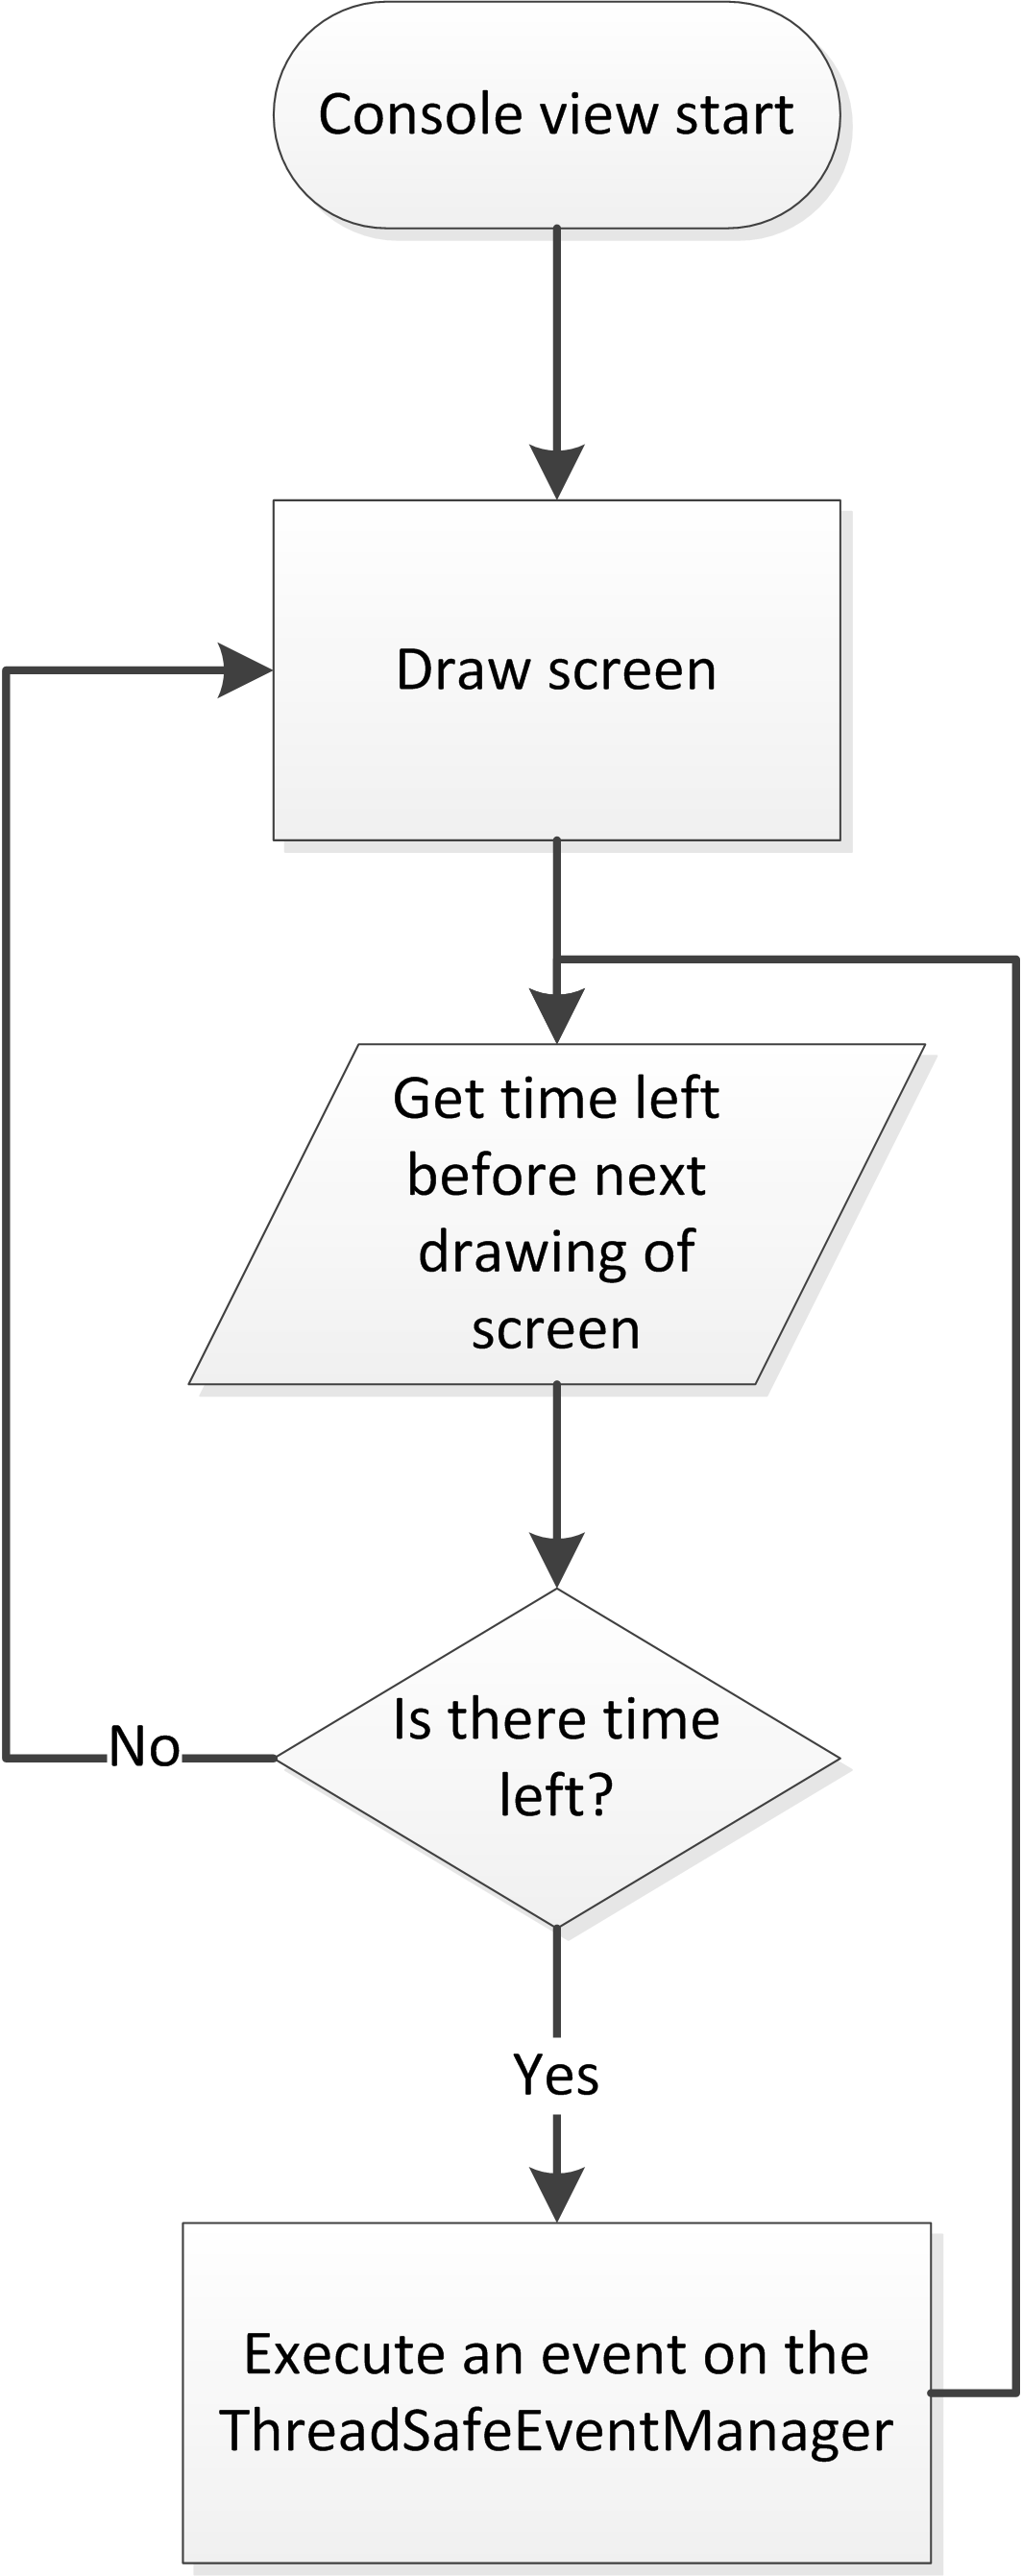
\includegraphics[width=0.4\textwidth]{ConsoleViewDrawingFlowChart}
\par\end{centering}

\caption{the sequence of the console view drawing process\label{fig:FlowOfConsole}}


\end{figure}


The console view works by drawing the screen, then -- if it has time
left before the next drawing is scheduled -- it will execute a single
event on the \texttt{ThreadSafeEventManager}. The view will continue
this process until either there are no events left to be executed
or the time is up and it is time for it to perform the next drawing
of the screen. In fig. \ref{fig:FlowOfConsole} an illustration of
this process is shown.

This provides the reference implementation with a very quickly updated
view as no time is wasted on the thread, since the view will continue
to update even when it is not drawing. Furthermore, by updating the
view data in a separate thread the engine core does not use its computation
power on handling this, which makes the engine more efficient overall.


\subsection{GOAL Program Implementation}

The GOAL program is designed to work directly with our reference implementation,
as it is just a showcase of what such a program might look like. It
will make assumptions about how the reference implementation works.
For instance, it will assume that there are entities called walls
that blocks movement. 

To see the commented source code of our GOAL program, see appendix
\ref{chap:GoalCodeAppendix}.


\subsubsection{Agent Decision}

A full flow chart of the goal program decision chart can be found
in appendix \ref{sec:GOALFlowChartAppendix}.

As can be seen from the flow chart, the agent will try to find packages
and bring them to a dropzone, if no such packages can be found or
if no dropzone is found, the agent will start exploring the entire
world.

The goal program operates with a few different notions; 
\begin{description}
\item [{Street}] The first notion is the notion of streets. A tile is a
street if it contains no wall types such as normal walls or impassableWalls
(map boundary walls). This means that the agent can move on this tile.
\item [{Route}] When an agent decides to move to a specific tile, it will
perform an \texttt{A{*}} search to find the shortest path to that
tile. The \texttt{A{*}} search (which is called \texttt{As} in the
GOAL / prolog code found in appendix \ref{chap:GoalCodeAppendix})
returns a route represented by a list of tiles the agent should follow
to reach the desired tile. Whenever the agent have no tasks of higher
priority (such as grabbing a package if it is standing on one), it
will pop a tile from the route and move onto it.
\end{description}
\begin{figure}
\begin{centering}
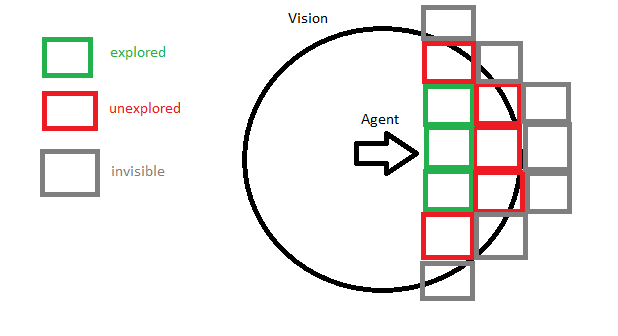
\includegraphics[width=0.8\textwidth]{VisionExploredGOALAgent}
\par\end{centering}

\caption{An image of an agent\textquoteright{}s vision and which it would determine
to be explored\label{fig:VisionExploredGoalAgent}}
\end{figure}

\begin{description}
\item [{Explored}] the agent\textquoteright{}s goal is to eventually have
all tiles explored as this means that it can determine whether all
packages have been picked up. The agent determines that a tile has
been explored if it has seen all its adjacent tiles (fig. \ref{fig:VisionExploredGoalAgent}
shows an image of this). No matter how much the agent explores, whenever
it uncovers a previously unexplored tile, it will see new tiles to
explore, unless the uncovered tile is a wall. This will continue until
a wall has been reached on all its paths. Uncovering a new tiles works
much like putting a carrot in front of a mule; it will always try
to catch up to the carrot, just as the agent will try to uncover unexplored
tiles.
\end{description}

\subsection*{Summary}

The reference implementation was designed as a reference for all the
features of the engine, as such it made heavy use of the extensions
that we implemented. This section only covered the view and the goal
program in details. This is because most of the reference implementation
consists of either declaring new agent/entity types or wiring all
the extensions together. As such, there was almost no business logic
involved which makes them rather uninteresting to explain in detail.

One part that the reference implementation does not cover which could
have been interesting was the notion of linked modules as explained
in \ref{sub:SysFeatEntities}. This could have been used in the reference
implementation but we did not choose to do so.

Overall the design of the reference implementation is very solid and
fulfills the goals we had for it, which were to be a showcase for
our engine.
